\documentclass{beamer}
%\documentclass{article}
%\usepackage[noxcolor]{beamerarticle}
\usepackage[ngerman]{babel}
\usepackage[utf8]{inputenc}
\usepackage{amsmath}
\usepackage{amsthm}
\usepackage{siunitx}
\usepackage{graphicx}
\usepackage{pgfplots}
\sisetup{locale = DE,
per-mode=fraction}
% Lade Beamer Stile
\usepackage{beamerthemesplit}
\usepackage{tcolorbox}
\usetheme{Rochester}
\usecolortheme{crane}


\title{2. Unterrichtseinheit zur Dynamik}
\subtitle{Arbeit und Energie}
\author{Heiko Schröter}
\date{\today}

\setbeamertemplate{enumerate item}{\alph{enumi})}

\begin{document}

\frame{\titlepage}

\frame
{
  \frametitle{Ziele für die heutige Unterrichtseinheit}
  \textbf{Mechanische Arbeit}
  \begin{itemize}
	\item Wie ist der Begriff mechanische Arbeit definiert?
	\item Welche Arten von mechanischer Arbeit gibt es?
	\item Wie hängen Arbeit und Energie zusammen?
	\item Der Energieerhaltungssatz der Mechanik?
	\item Welchen Einfluss hat eine mechanische Hilfe, ein Bauteil oder eine Maschine auf die Arbeit?
	\item Wie ist die Leistung $P$ definiert?
  \end{itemize}
}

\frame[allowframebreaks]
{
  \frametitle{Mechanische Arbeit}
\begin{block}{}
Mechanische Arbeit wird verrichtet, wenn eine Kraft gegen einen Widerstand längs eines zurückgelegten Weges wirkt.
\end{block}
\begin{block}{}
Die mechanische Arbeit $W$ wird berechnet als Produkt aus der in Richtung des Weges wirkenden Kraft $F$ und dem zurückgelegten Weg $s$.\\
$W=F\cdot s$
\end{block}
Die SI-Einheit der Arbeit $W$ ist:
$[W]=[F]\cdot[s]=\SI{1}{\newton\meter}=\SI{1}{\joule}$
    \begin{figure}
	  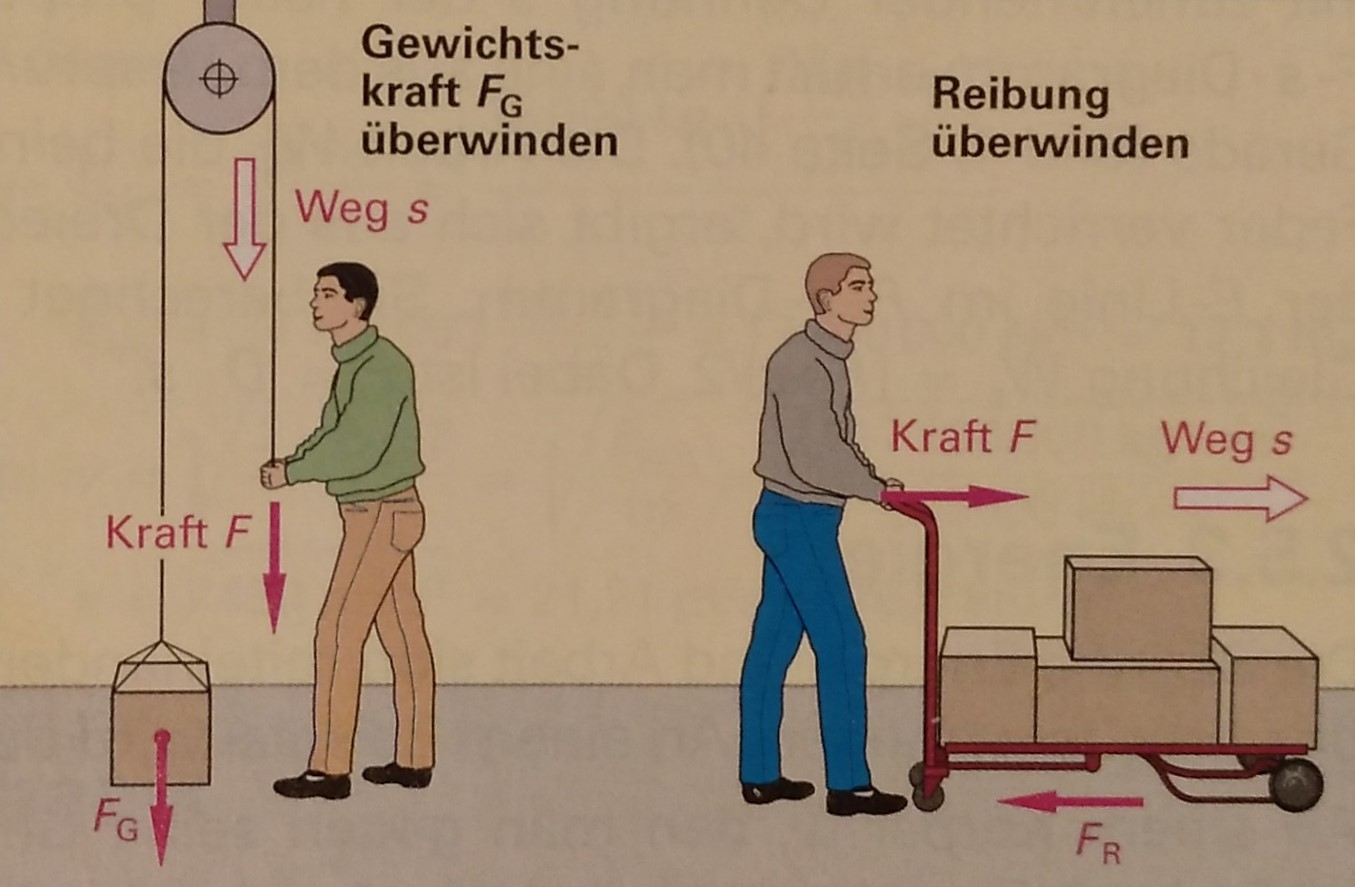
\includegraphics[width=0.7\textwidth]{Arbeit}
	  \vspace{-3mm}
	  \caption{Verrichten mechanischer Arbeit}
   \end{figure}
Die genannte Gleichung $W=F\cdot s$ gilt nur, wenn die Kraft $F$ entlang des Weges $s$ konstant bleibt.
}

\frame
{
  \frametitle{Arten mechanischer Arbeit}
  \begin{block}{Hubarbeit}
	\begin{align}
	W_H=F\cdot s=F_G\cdot h=m\cdot g\cdot h
	\end{align}
  \end{block}
  \textbf{Beispiel:} Welche mechanische Arbeit (Hubarbeit) wird beim anheben einer Palette mit $\SI{1520}{\kilo\gram}$ auf die Höhe der Ladefläche eines Lastwagens von $\SI{1,20}{\meter}$ verrichtet?\\
  \textbf{Lösung:}
  \begin{align*}
  W_H&=m\cdot g\cdot h=\SI{1520}{\kilo\gram}\cdot \SI{9,81}{\meter\square\second}\cdot \SI{1,20}{\meter}\\
  &=\SI{17893}{\newton\meter}=\SI{17,9}{\kilo\joule}
  \end{align*}
}

\frame
{
  \frametitle{Arten mechanischer Arbeit}
  \begin{block}{Reibungsarbeit}
	\begin{align}
	W_R=F_R\cdot s=\mu\cdot F_N\cdot s
	\end{align}
  \end{block}
  \textbf{Reibungsarbeit.} Bei der gleichförmig geradlinigen Bewegung eines Körpers auf horizontaler Unterlage muss die Reibungskraft $F_R$ entlang des Weges $s$ überwunden werden. Die Reibungskraft $F_R$ ist: $F_R=\mu\cdot F_N$
}

\frame
{
  \frametitle{Arten mechanischer Arbeit}
  \begin{block}{Beschleunigungsarbeit}
	\begin{align}
	W_B=F_B\cdot s=m\cdot a\cdot s\\
	W_B=m\cdot\dfrac{(a\cdot t)^{2}}{2}\\
	W_B=\dfrac{1}{2}\cdot m\cdot v^{2}
	\end{align}
  \end{block}
  \textbf{Beschleunigungsarbeit.} Um einen Körper längs eines Weges $s$ konstant zu beschleunigen, muss nach dem Grundgesetz der Dynamik die Kraft $F_B$ wirken.
}

\frame
{
  \frametitle{Arten mechanischer Arbeit}
  \begin{block}{Spannarbeit}
	\begin{align}
	W_S=\dfrac{(F\cdot s)}{2}=\dfrac{1}{2}\cdot D\cdot s^{2}\\
	\end{align}
  \end{block}
  \textbf{Spannarbeit.} Beim spannen einer Feder nimmt die Kraft $F$ mit zunehmender Dehnung $s$ der Feder proportional zu. Im F-s-Diagramm erhält man eine aus dem Ursprung ansteigende Gerade. Die Arbeit $W_s$, die beim Spannen der Feder verrichtet wird, ergibt sich aus der Dreiecksfläche unter der F-Linie im F-s-Diagramm.
}

\frame[allowframebreaks]
{
  \frametitle{Energie}
Die Begriffe Energie und Arbeit sind miteinander verknüpft. Als Energie bezeichnet man in der Physik das Arbeitsvermögen.
    \begin{figure}
	  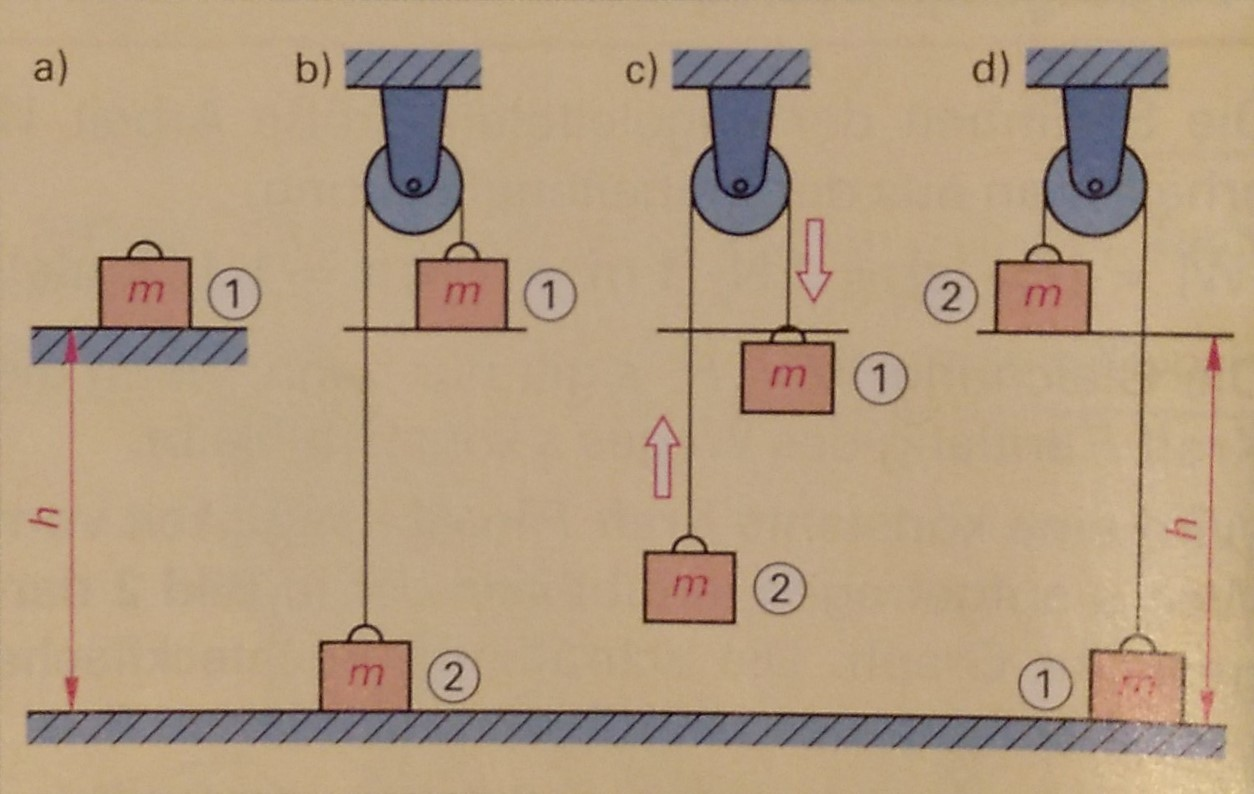
\includegraphics[width=0.7\textwidth]{Energie}
	  \vspace{-3mm}
	  \caption{Zusammenhang von Arbeit und Energie}
   \end{figure}
  \begin{block}{Potentielle Energie}
Das Arbeitsvermögen, das ein Körper aufgrund seiner Hochlage besitzt, wird als potentielle Hubenergie, kurz potentielle Energie oder Lageenergie bezeichnet.	
	\begin{align}
	E_{pot}=W_H=m\cdot g\cdot h
	\end{align} 
  \end{block}\newpage
    \begin{block}{Potentielle Spannenrgie}
Auch beim Spannen einer Feder bleibt die geleistete Spannarbeit $W_S$ als potentielle Energie der gespannten Feder erhalten.	
	\begin{align}
	E_{pot}=W_S=\dfrac{1}{2}\cdot D\cdot s^{2}
	\end{align} 
  \end{block}
  \textbf{Beispiel:} Die in einem Ventil eingebaute Rückstellfeder mit der Federkonstante $D=\SI{5000}{\newton\per\meter}$ ist mit der Energie $E_{pot}=\SI{3,8}{\joule}$ gespannt.\\
  \begin{enumerate}
  	\item Wie groß ist der Federweg $s$, um den die Feder zusammengedrückt ist?
  	\item Wie groß ist die dazu aufzuwendende Spannkraft?
  \end{enumerate}
  \textbf{Lösung:}
  \begin{enumerate}
  \item
  \begin{align*}
  E_{pot}=W_S=\dfrac{1}{2}\cdot D\cdot s^{2}\Rightarrow s&=\sqrt{\dfrac{2\cdot E_{pot}}{D}}\\
  &=\sqrt{\dfrac{2\cdot \SI{3,8}{\joule}}{\SI{5000}{\newton\per\meter}}}\\
  &=\SI{0,039}{\meter}=\SI{3,9}{\centi\meter}
  \end{align*}
  \item
    \begin{align*}
	F&=D\cdot s=\SI{5000}{\newton\per\meter}\cdot\SI{0,039}{\meter}\\
	&=\SI{195}{\newton}
  \end{align*}
  \end{enumerate}
  
  \begin{block}{Kinetische Energie}
Lässt man einen Körper frei fallen, so erfährt er durch seine Gewichtskraft eine gleichmäßige Beschleunigung und seine Geschwindigkeit steigt fortlaufend an.	
	\begin{align}
	E_{kin}=W_B=\dfrac{1}{2}\cdot m\cdot v^{2}
	\end{align}
  \end{block}
  Analog zur Speicherung der Hubarbeit $W_H$ als Lageenergie $E_{pot}$, wird beim Fallen verrichtete Beschleunigungsarbeit $W_B$ als Arbeitsfähigkeit im bewegten Körper gespeichert.\\
  Man bezeichnet das Arbeitsvermögen, das ein Körper aufgrund seiner Geschwindigkeit hat, als Bewegungsenergie oder kinetische Energie.
}
  \textbf{Beispiel:} Ein Gefahrguttransporter mit einer Masse von \SI{38}{\tonne} fährt auf der Autobahn mit der überhöhten Geschwindigkeit von \SI{108}{\kilo\meter\per\hour}.\\
  \begin{enumerate}
  	\item Berechnen Sie die kinetische Energie $E_{kin}$ des Lastzuges.?
  	\item Mit welcher Geschwindigkeit $v$ fährt der Gefahrguttransporter, wenn seine kinetische Energie $E_{kin}$ durch bremsen halbiert wurde?
  \end{enumerate}
  \newpage
  \textbf{Lösung:}
  \begin{enumerate}
  \item
  \begin{align*}
	E_{kin}&=\dfrac{1}{2}\cdot m\cdot v^{2}=\dfrac{\SI{38000}{\kilo\gram}\cdot \left(\dfrac{108}{3,6}\dfrac{\si{\meter}}{\si{\second}}\right)^{2}}{2}\\
	&=\SI{17100000}{\kilo\gram\square\metre\per\square\second}=\SI{17100000}{\newton\meter}=\SI{17,1}{\mega\joule}
  \end{align*}
  \item
    \begin{align*}
	v&=\sqrt{\dfrac{2\cdot \frac{E_{kin}}{2}}{m}}=\sqrt{\dfrac{E_{kin}}{m}}=\sqrt{\dfrac{\SI{17100000}{\kilo\gram\square\metre\per\square\second}}{\SI{38000}{\kilo\gram}}}\\
	&=\sqrt{\SI{450}{\square\meter\per\square\second}}=\SI{21,21}{\meter\per\second}=\SI{76,4}{\kilo\meter\hour}
  \end{align*}
  \end{enumerate}

\frame[allowframebreaks]
{
  \frametitle{Energieerhaltungssatz der Mechanik}
\begin{block}{Energieerhaltungssatz der Mechanik}
Bei mechanischen Vorgängen wird potentielle Energie in kinetische Energie bzw. kinetische Energie in potentielle Energie umgewandelt. Wirken dabei nur die Schwerkraft und Federkräfte, bleibt die Summe von potentieller und kinetischer Energie konstant.\\
$E_{Ges}=E_{pot}+E_{kin}=$konstant
\end{block}

    \begin{figure}
	  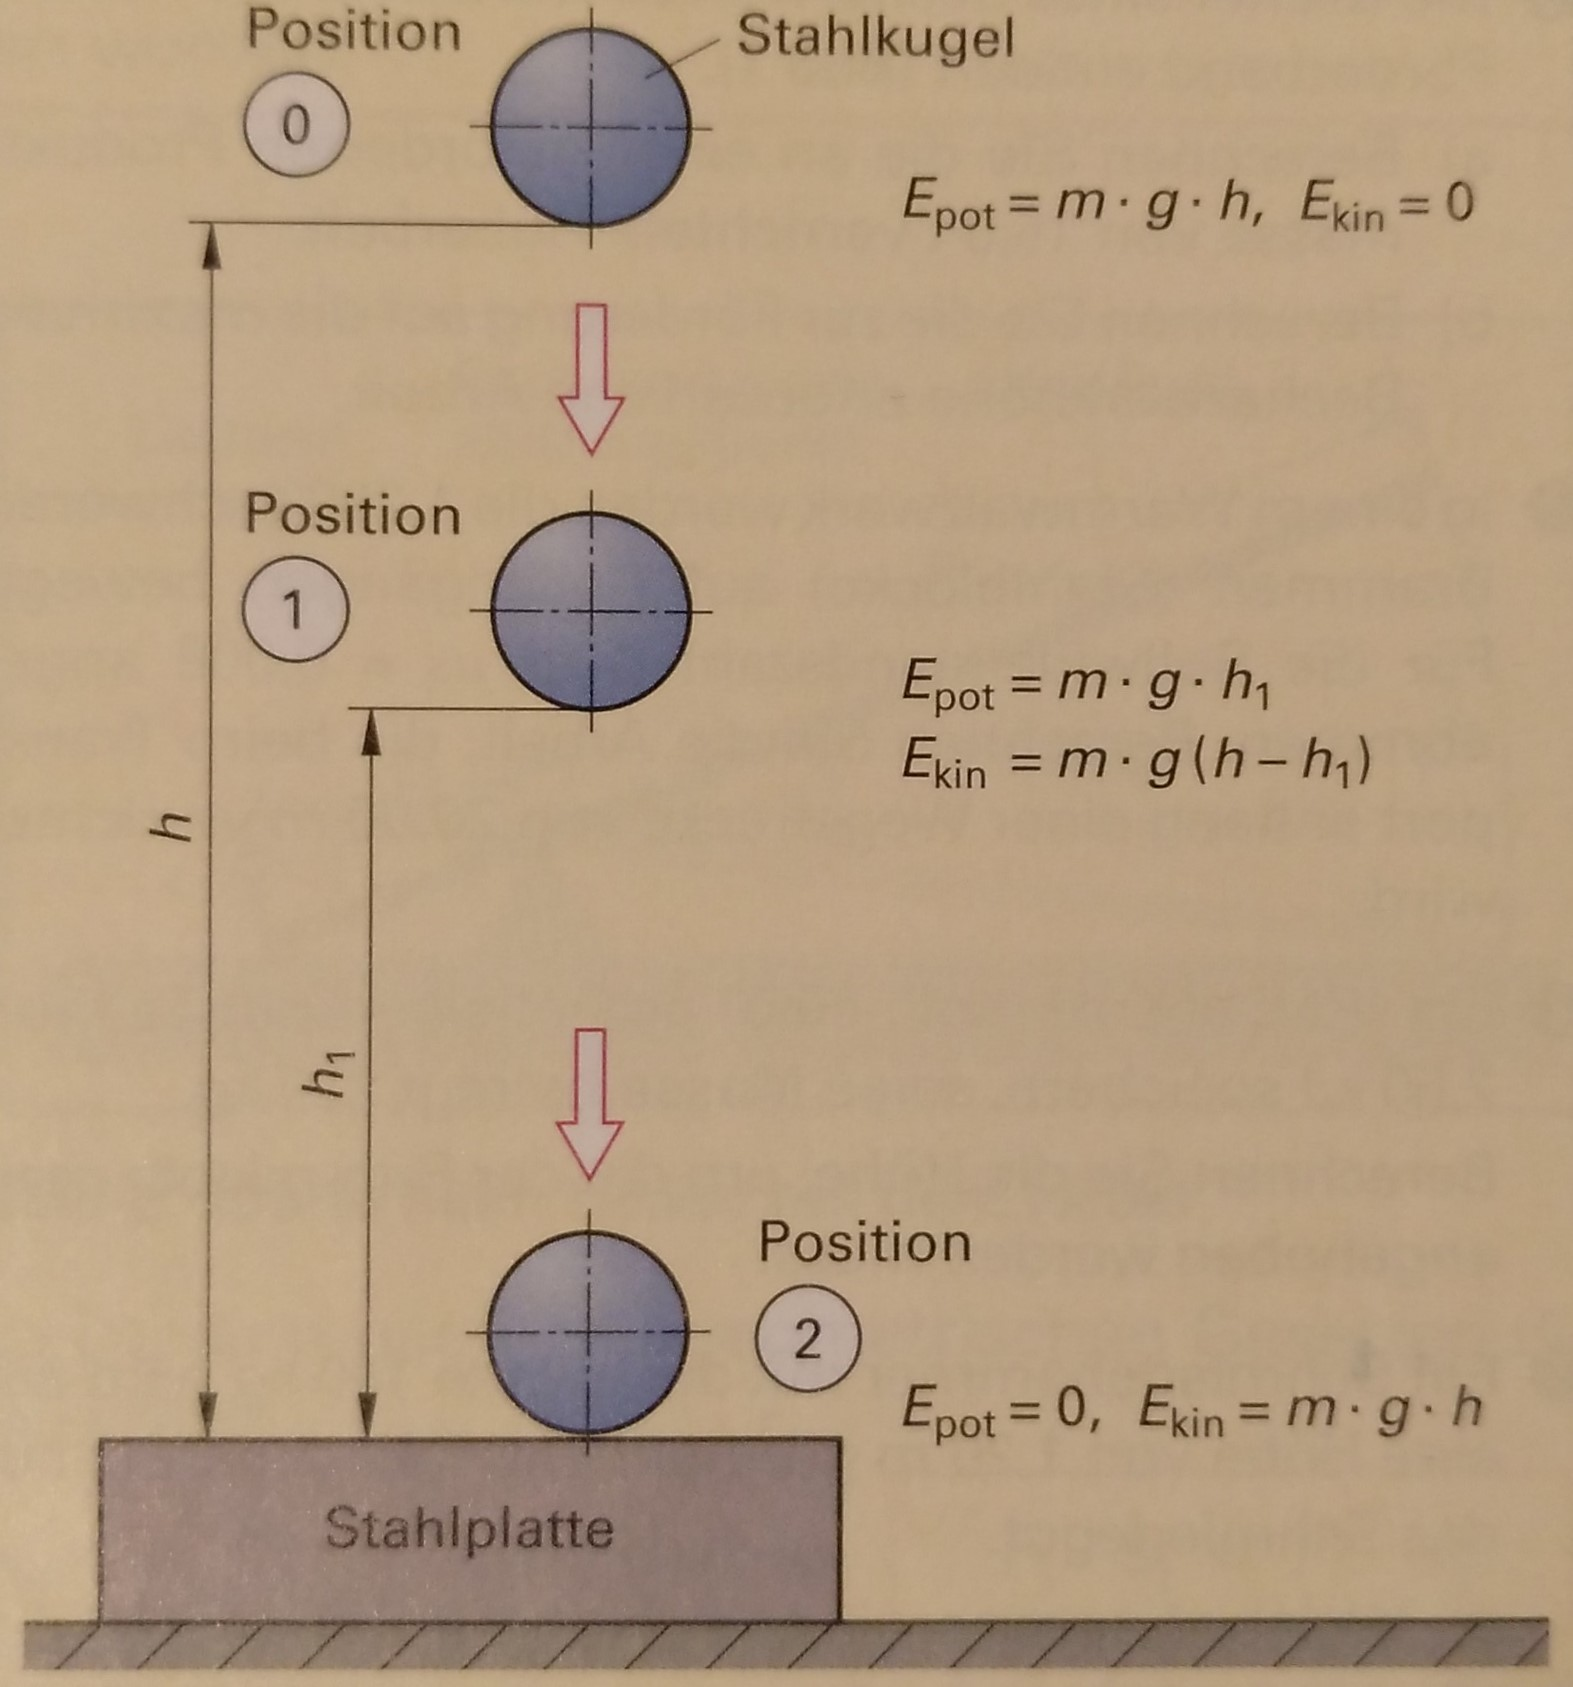
\includegraphics[width=0.5\textwidth]{Energieformen}
	  \vspace{-3mm}
	  \caption{Umwandlung der Energieformen beim Fallen}
   \end{figure}

}

\frame[allowframebreaks]
{
  \frametitle{Mechanische Hilfen und Bauteile}
\begin{block}{goldene Regel der Mechanik}
Durch eine mechanische Hilfe, ein Bauteil oder eine Maschine kann keine Arbeit gespart werden. Was an Kraft gespart wird muss an Weg zugegeben werden.\\
\end{block}
\begin{exampleblock}{geneigte Ebene}
    \begin{figure}
	  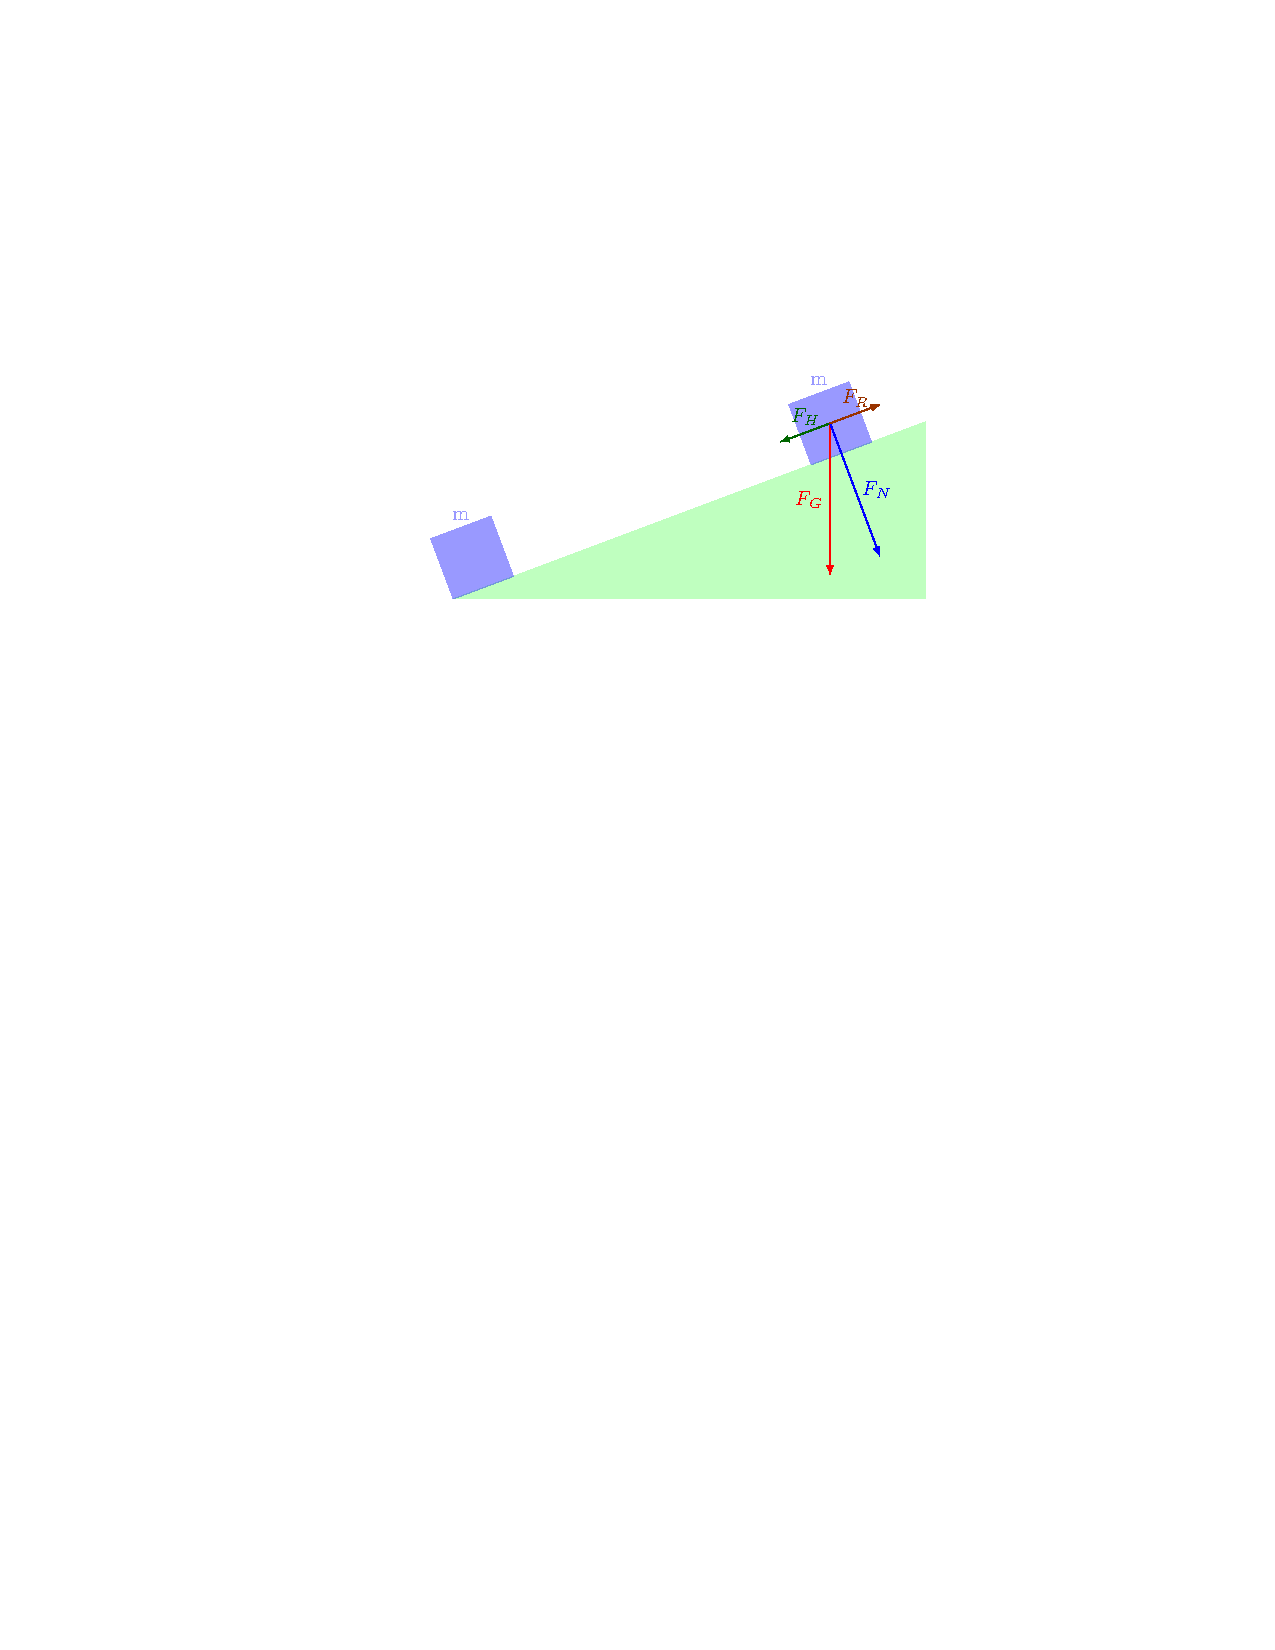
\includegraphics[width=0.35\textwidth]{geneigte_Ebene}
	  \vspace{-3mm}
	  \caption{Kräfte an der Last einer geneigten Ebene}
	  %$W_Z=m\cdot g\cdot\sin \alpha\cdot s$
   \end{figure}
\end{exampleblock}
\begin{exampleblock}{Hebel}
    \begin{figure}
	  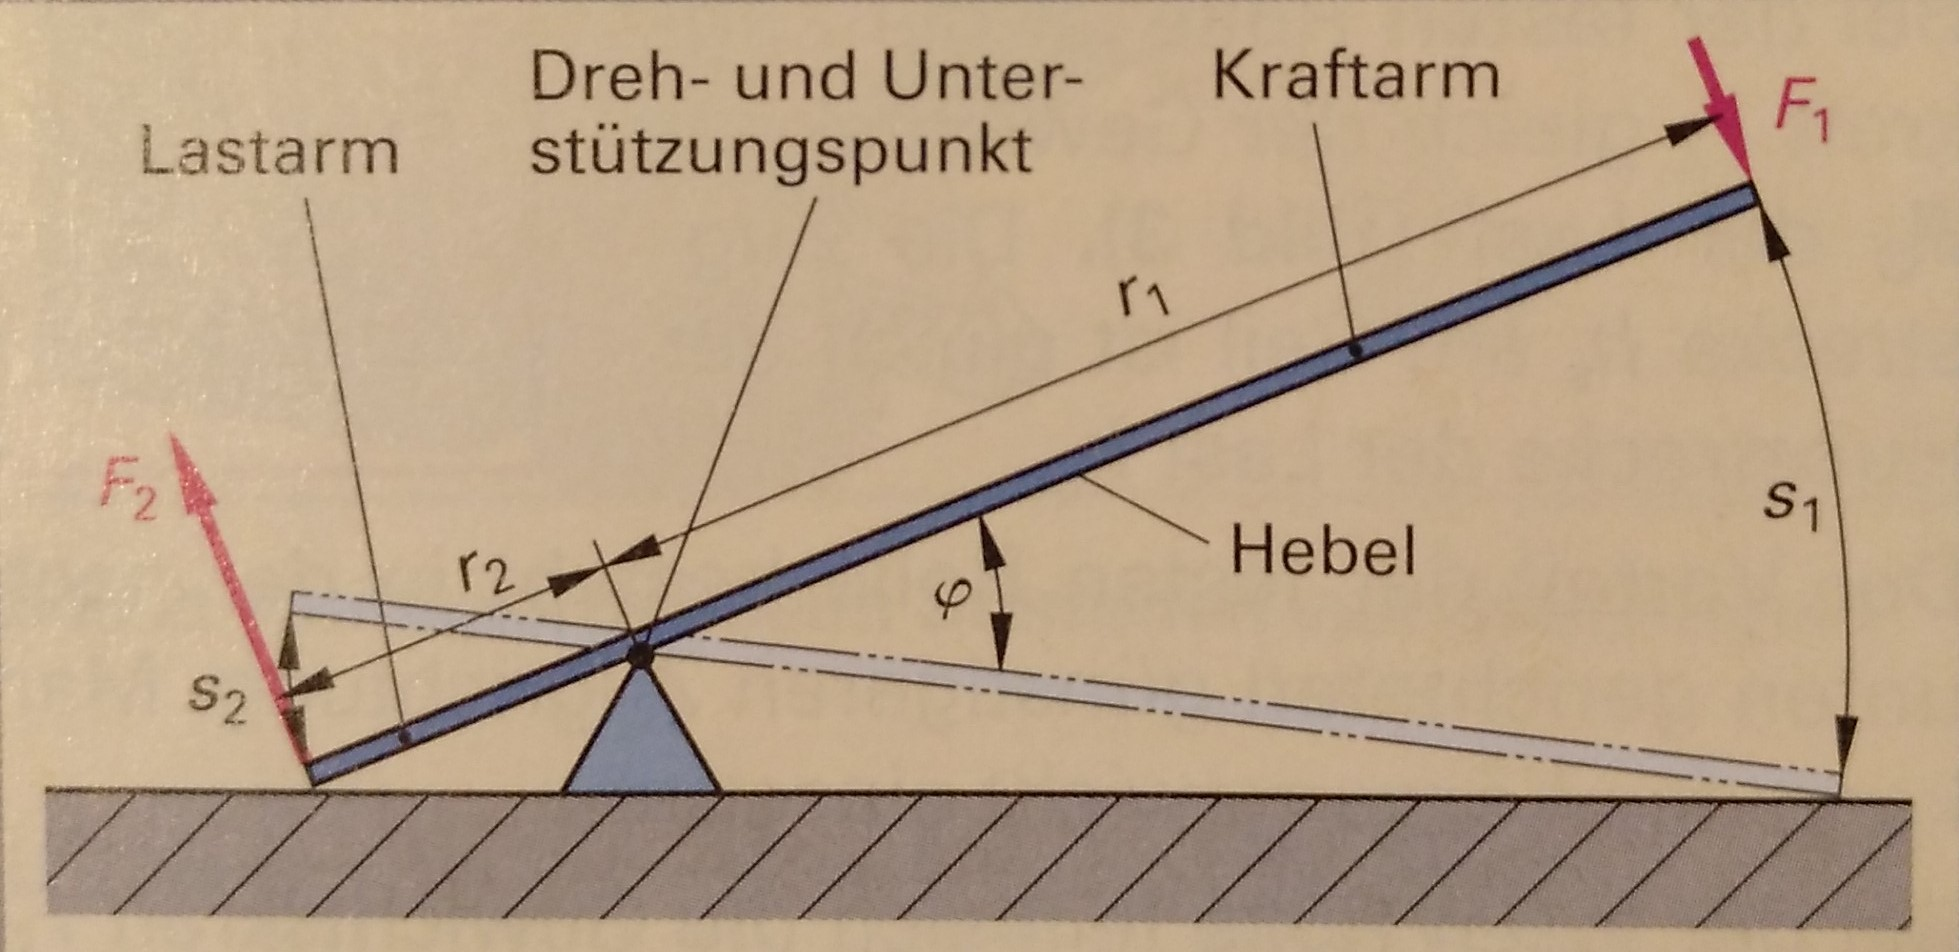
\includegraphics[width=0.5\textwidth]{Hebel}
	  \vspace{-3mm}
	  \caption{Kräfte beim Heben mit dem Hebel}
   \end{figure}
   $F_1\cdot s_1=F_2\cdot s_2$
\end{exampleblock} \newpage
\begin{exampleblock}{Schraube}
    \begin{figure}
	  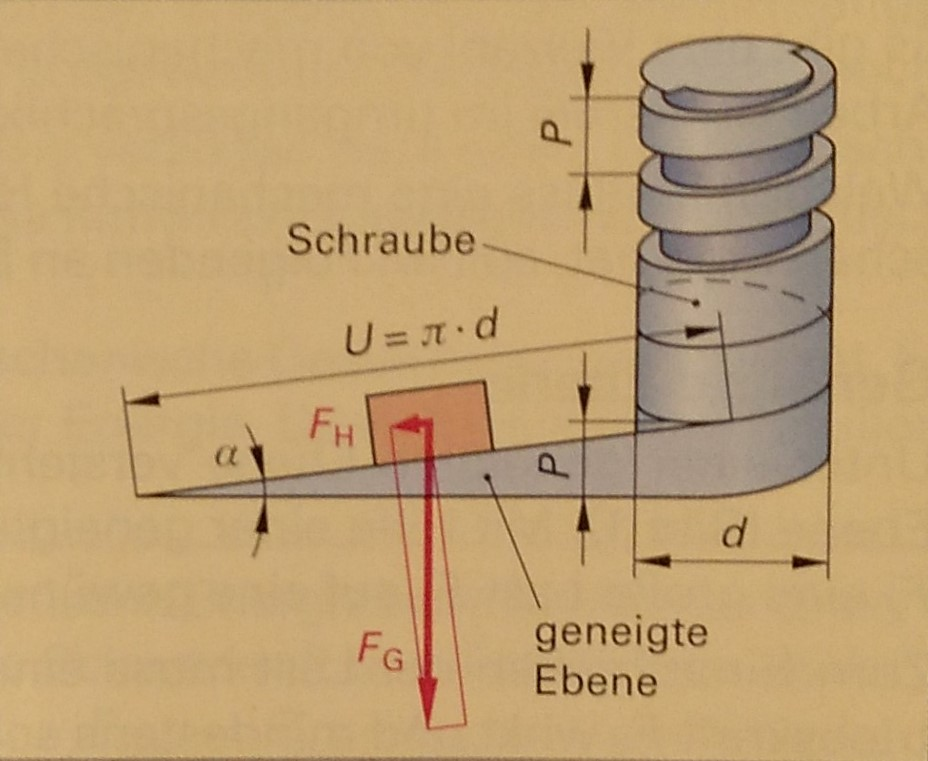
\includegraphics[width=0.45\textwidth]{Schraube}
	  \vspace{-3mm}
	  \caption{Das Schraubengewinde als aufgewickelte, geneigte Ebene}
   \end{figure}
   %$F_H=F_G\cdot \sin \alpha=F_G\cdot\dfrac{P}{U}$
\end{exampleblock} \newpage
\begin{exampleblock}{Schraube}
    \begin{figure}
	  \includegraphics[width=0.4\textwidth]{Schraubenschlüssel2}
	  \vspace{-3mm}
	  \caption{Kräfte beim Anziehen einer Schraube mit dem Schraubenschlüssel}
   \end{figure}
   $F_H\cdot (2\pi\cdot l)=F_G\cdot \sin P$
\end{exampleblock} \newpage
\begin{exampleblock}{Feste Rolle und lose Rolle}
    \begin{figure}
	  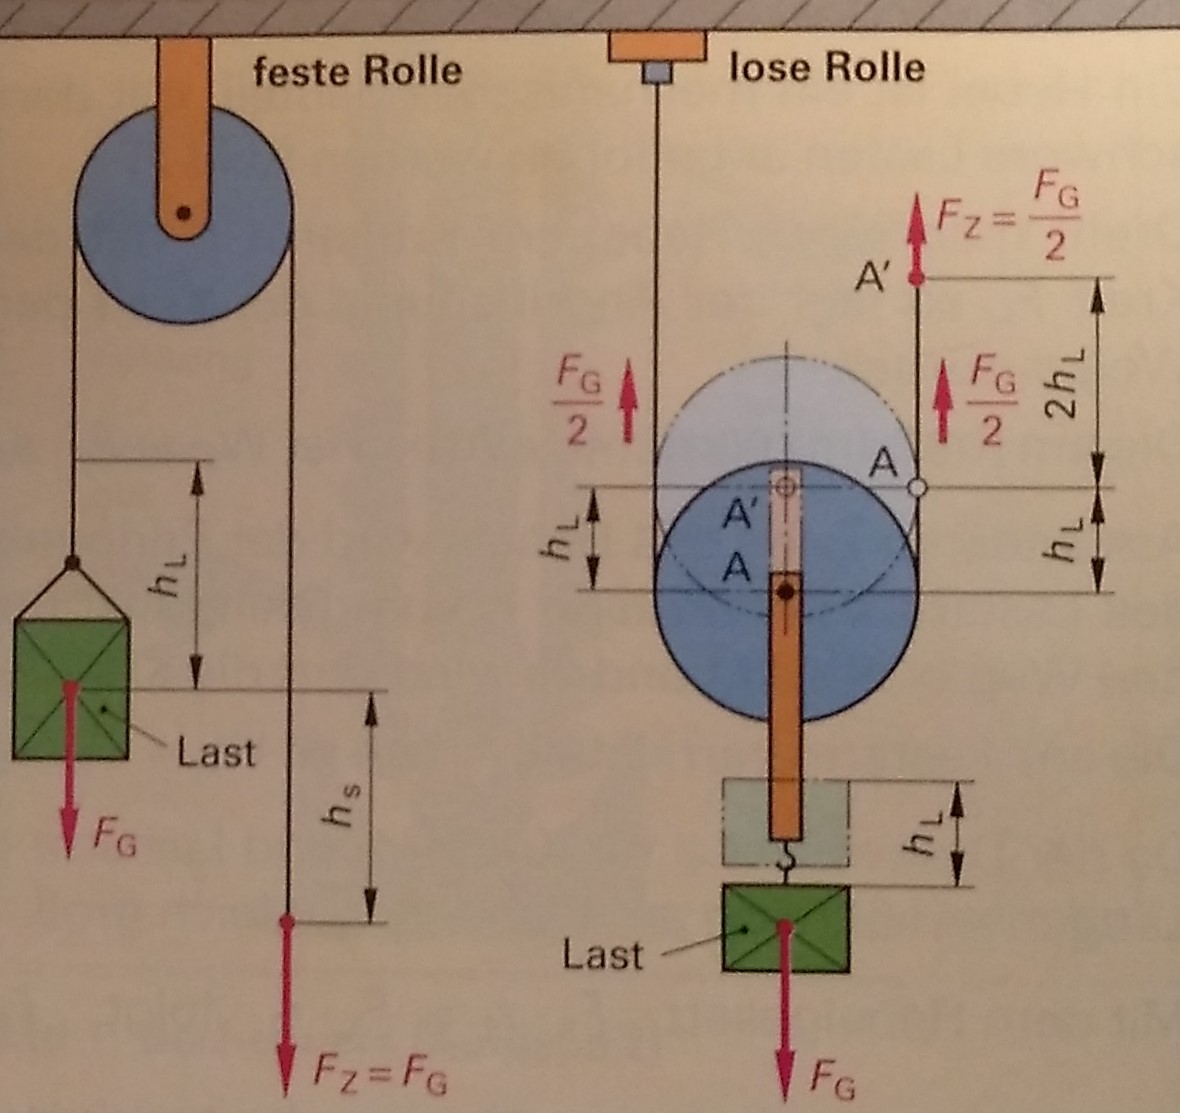
\includegraphics[width=0.45\textwidth]{Rolle}
	  \vspace{-3mm}
	  \caption{Kräfte bei der festen Rolle und bei der losen Rolle}
   \end{figure}
   %$F_H=F_G\cdot \sin \alpha=F_G\cdot\dfrac{P}{U}$
\end{exampleblock}
}
\frame[allowframebreaks]
{
  \frametitle{Leistung}
\begin{block}{Definition}
Die Leistung $P$ ist der Quotient aus der verrichteten Arbeit $W$ und der dazugehörigen Zeit $t$.\\
$P=\dfrac{W}{t}$
\end{block}
Die SI-Einheit der Leistung $P$ ergibt sich aus der Einheitengleichung zu \si{\newton\meter\per\second} oder \si{\joule\per\second}. Sie wird \textbf{Watt}\footnote{James Watt: englischer Physiker (1736 bis 1819}  (Einheitszeichen $W$) genannt. 
	\begin{tcolorbox}	  
	  $[P]=\dfrac{[W]}{[t]}=\dfrac{\SI{1}{\newton\meter}}{\SI{1}{\second}}=\SI{1}{\joule\per\second}=\SI{1}{\watt}$ (Watt)
	\end{tcolorbox}
}

\frame
{
  \frametitle{Übungsaufgabeaufgabe Arbeit}
\uncover<1->
{
Bei einem Wasserkraftwerk werden tagsüber \SI{100000}{\cubic\meter} Wasser dem oberen Rückhaltebecken entnommen. Dabei wird den Turbinen eine Arbeit von \SI{40000}{\kilo\watt\hour} zugeführt. Wie groß ist die Fallhöhe ($g=\SI{9,81}{\meter\per\square\second}$, Strömungsverluste bleiben unberücksichtigt)?\\
}
\uncover<2->
{
\textbf{Lösung:}	
	\begin{align*}
	\Delta W&=F_s\cdot \Delta s\Rightarrow\Delta s=\dfrac{\Delta W}{F_s}\Rightarrow\Delta s=\dfrac{\Delta W}{m\cdot g}\\
	\Delta s&=\dfrac{\SI{40000}{\kilo\watt\hour}}{100\cdot 10^6\si{\kilo\gram}\cdot \SI{9,81}{\meter\per\square\second}}=\dfrac{4\cdot 10^7\cdot 3600\si{\watt\second}}{100\cdot 10^6\si{\kilo\gram}\cdot \SI{9,81}{\meter\per\square\second}}\\
	\Delta s&\approx\SI{147}{\meter}
	\end{align*}
}
}

\frame
{
  \frametitle{Übungsaufgabeaufgabe Leistung}
\uncover<1->
{
Ein Aufzug soll mit der Kraft von \SI{1000}{\newton} angetrieben werden und dabei eine Geschwindigkeit von \SI{2}{\meter\per\second} haben. Berechnen Sie die erforderliche Leistung.\\
}
\uncover<2->
{
\textbf{Lösung:}	
	\begin{align*}
	P=F_s\cdot v=\SI{1000}{\newton}\cdot\SI{2}{\meter\per\second}=\SI{2000}{\newton\meter\per\second}=\SI{2}{\kilo\watt}
	\end{align*}
}
}

\frame
{
  \frametitle{Übungsaufgabeaufgabe Leistung}
\uncover<1->
{
Ein Elektroauto muss eine Reibungskraft von \SI{400}{\newton} überwinden und soll eine Geschwindigkeit von \SI{60}{\kilo\meter\per\hour} haben. Wie groß muss die erforderliche Antriebsleistung sein?\\
}
\uncover<2->
{
\textbf{Lösung:}	
	\begin{align*}
	P&=F_s\cdot v=\SI{400}{\newton}\cdot\SI{60}{\kilo\meter\per\hour}=\SI{400}{\newton}\cdot\dfrac{\SI{60000}{\meter}}{\SI{3600}{\second}}\\&=\SI{6667}{\newton\meter\per\second}=\SI{6,667}{\kilo\watt}
	\end{align*}
}
}
\end{document}
